\documentclass[12pt]{article}                   % Začátek dokumentu
\usepackage{../../MFFStyle}                     % Import stylu

\begin{document}
\begin{priklad}[5.1]
	Podrobně odvoďte a sestrojte přirozený kubický spline $S(x)$ interpolující funkci $f(x)$ danou tabulkou
	\begin{center}
		\begin{tabular}{|l|l|l|l|l|}
			\hline
			$i$      & 0 & 1 & 2 & 3 \\ \hline
			$x_i$    & 0 & 1 & 2 & 3 \\ \hline
			$f(x_i)$ & 0 & 1 & 0 & 0 \\ \hline
		\end{tabular}
	\end{center}
	Dále vypočtěte hodnotu $S(1.5)$.

	\begin{reseni}
		Jelikož chceme přirozený spline, tak $S''(x_0) = S''(x_3) = 0$. Z přednášky víme, že
		$$ \begin{pmatrix} 4 & 1 \\ 1 & 4 \end{pmatrix} \begin{pmatrix} S''(x_1) \\ S''(x_2) \end{pmatrix} = \begin{pmatrix} f(x_0) - 2f(x_1) + f(x_2) \\ f(x_1) - 2f(x_2) + f(x_3) \end{pmatrix} = \begin{pmatrix} -2 \\ 1 \end{pmatrix} $$
		Odečtením čtyřnásobku jedné rovnice od druhé získáme $S''(x_1) = -\frac{18}{5}$ a $S''(x_2) = \frac{12}{5}$. To pak můžeme dosadit do odvození z přednášky:{\tiny
		$$ S|_{[x_i, x_{i+1}]} = \frac{(x - x_i)^3}{6h}S''(x_{i+1}) + \frac{(x_{i+1} - x)^3}{6h}S''(x_i) + \(\frac{f(x_{i+1}) - f(x_i)}{h} - \frac{h}{6}\(S''(x_{i+1}) - S''(x_i)\)\)(x - x_i) + f(x_i) - \frac{h^2}{6}S''(x_i) $$
		$$ S|_{[0, 1]} = \frac{(x - 0)^3}{6·1}\(-\frac{18}{5}\) + \frac{(1 - x)^3}{6·1}0 + \(\frac{1 - 0}{1} - \frac{1}{6}\(-\frac{18}{5} - 0\)\)(x - 0) + 0 - \frac{1^2}{6}0 = \frac{8}{5}x - \frac{3}{5}x^3 $$
		$$ S|_{[1, 2]} = \frac{(x - 1)^3}{6·1}\frac{12}{5} + \frac{(2 - x)^3}{6·1}\(-\frac{18}{5}\) + \(\frac{0 - 1}{1} - \frac{1}{6}\(\frac{12}{5} + \frac{18}{5}\)\)(x - 1) + 1 - \frac{1^2}{6}\(-\frac{18}{5}\) = x^3 - \frac{24}{5}x^2 + \frac{32}{5}x - \frac{8}{5} $$
		$$ S|_{[2, 3]} = \frac{(x - 2)^3}{6·1}0 + \frac{(3 - x)^3}{6·1}\frac{12}{5} + \(\frac{0 - 0}{1} - \frac{1}{6}\(0 - \frac{12}{5}\)\)(x - 2) + 0 - \frac{1^2}{6}\frac{12}{5} = -\frac{2}{5}x^3 + \frac{18}{5}x^2 - \frac{52}{5}x + \frac{48}{5} $$
	}
		\begin{center}
			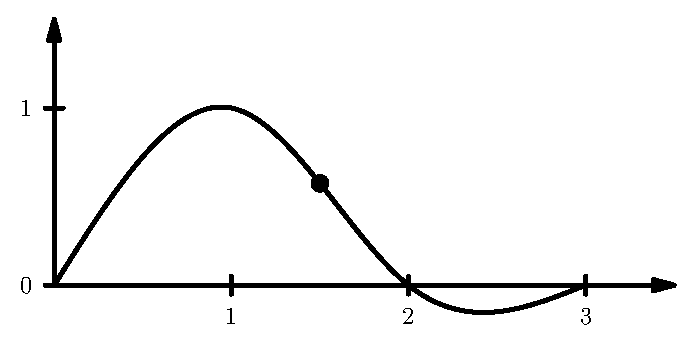
\includegraphics{spline.eps}
		\end{center}

		$$ S(1.5) = 1.5^3 - \frac{24}{5}1.5^2 + \frac{32}{5}1.5 - \frac{8}{5} = \frac{23}{40} = 0.575. $$
	\end{reseni}
\end{priklad}

\end{document}
